\documentclass{article}
% translate with >> pdflatex -shell-escape <file>

% This file is an extract of the PGFPLOTS manual, copyright by Christian Feuersaenger.
% 
% Feel free to use it as long as you cite the pgfplots manual properly.
%
% See
%   http://pgfplots.sourceforge.net/pgfplots.pdf
% for the complete manual.
%
% Any required input files (for <plot table> or <plot file> or the table package) can be downloaded
% at
% http://www.ctan.org/tex-archive/graphics/pgf/contrib/pgfplots/doc/latex/
% and
% http://www.ctan.org/tex-archive/graphics/pgf/contrib/pgfplots/doc/latex/plotdata/

\usepackage{pgfplots}
\pgfplotsset{compat=newest}

\pagestyle{empty}

\begin{document}
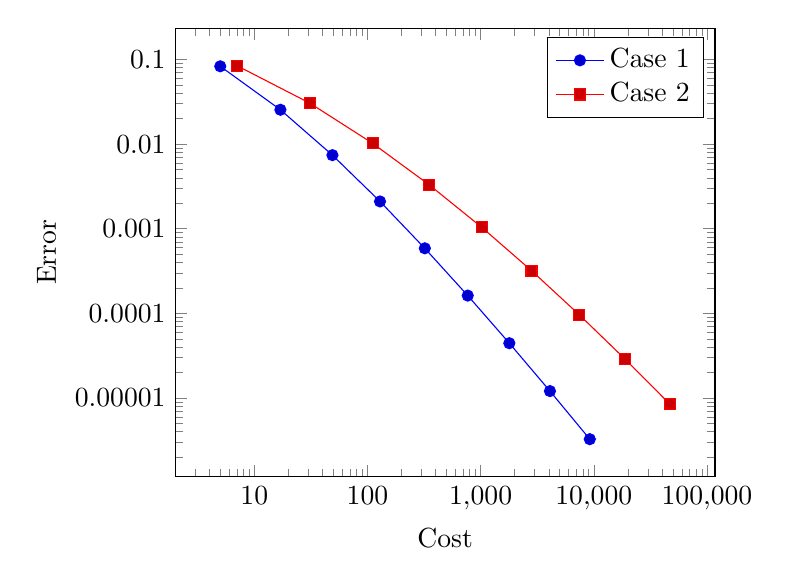
\begin{tikzpicture}
\begin{loglogaxis}[
	log ticks with fixed point,
	xlabel=Cost,ylabel=Error]
\addplot coordinates {
	(5,     8.31160034e-02)
	(17,    2.54685628e-02)
	(49,    7.40715288e-03)
	(129,   2.10192154e-03)
	(321,   5.87352989e-04)
	(769,   1.62269942e-04)
	(1793,  4.44248889e-05)
	(4097,  1.20714122e-05)
	(9217,  3.26101452e-06)
};
\addplot coordinates {
	(7,     8.47178381e-02)
	(31,    3.04409349e-02)
	(111,   1.02214539e-02)
	(351,   3.30346265e-03)
	(1023,  1.03886535e-03)
	(2815,  3.19646457e-04)
	(7423,  9.65789766e-05)
	(18943, 2.87339125e-05)
	(47103, 8.43749881e-06)
};
\legend{Case 1,Case 2}
\end{loglogaxis}
\end{tikzpicture}
\end{document}
